\section{Introduction}
\label{sec:intro}

% Climate and weather models are expensive, and we really want ensembles
Weather and climate prediction requires the integration of a computational
forecast model, derived from the fundamental equations of motion and initialized
with an estimate of the present-day system state (e.g., temperature, wind speeds,
etc.).
Our knowledge of these initial conditions is imperfect, however, and the governing
equations contain necessary approximations of reality.
Thus, reliable climate projections and weather forecasts require an
ensemble of numerical model integrations, where each ensemble member is
initialized by sampling from a prior distribution
representing our uncertainty in the present system state.
This process comes at an immense computational cost.
On the one hand, it is desirable to increase the credibility of the underlying
numerical model as much as possible,
for instance by increasing model grid resolution or by explicitly
simulating as many coupled components (e.g., atmosphere, land, ocean, ice) as
possible.
On the other hand, producing an ensemble with reliable statistical significance
requires integrating the underlying numerical model many times; usually
$\mathcal{O}(10-100)$ in practice, but ideally $>1,000$.
Therefore, the resulting computational costs require practitioners to trade between the
fidelity of the numerical model and the size of the ensemble.

% Surrogate modeling an encouraging path, and with increased computing power,
% ML, NNs ...
A current line of research for enabling statistical forecasting with an
expensive numerical model is \textit{surrogate modeling}.
The general approach involves deriving a surrogate model or emulator which
can be evaluated much faster than the original numerical model, while
capturing the dynamics of the underlying system ``accurately enough'' for
reliable prediction.
Historically, engineering applications have made use of
reduced order models \citep{moore_linear_2022},
polynomial chaos expansions,
...
More recently, advances in computing power, the explosion of freely available data, and
more widespread usage of General Purpose Graphics Processing Units (GPGPUs) has
encouraged the exploration of using Machine Learning (ML) methods like neural
networks for the emulation task.
Within the broad scope of weather forecasting and climate projection
applications, many \red{research groups} have begun to develop
neural network-based surrogate models to represent the
general circulation of the atmosphere and oceans, see \cref{table:all_the_emulators}.


\begin{table}[]
\caption{
    Recent work using neural networks to emulate processes relevant to weather
    forecasting and climate projection.
}
\label{table:all_the_emulators}

{\footnotesize
\begin{tabular}{c|c|c|c|c|l}
System     & Data Source             & \begin{tabular}[c]{@{}c@{}}Process or\\ Variable\end{tabular} & \begin{tabular}[c]{@{}c@{}}Horizontal\\ Resolution\end{tabular} & Timestep & Citation                                            \\
\hline
Atmosphere & ``Idealized GCM''       &                                                               &                                                                 &          & \citep{scher_weather_2019}       \\
           & 2 Layer QG              &                                                               &                                                                 &          & \citep{chattopadhyay_deep_2020}  \\
           & SPEEDY                  &                                                               &                                                                 &          & \citep{arcomano_machine_2020}    \\
           & WRF North America       &                                                               &                                                                 &          & \citep{maulik_efficient_2022}    \\
           & ERA5                    &                                                               &                                                                 &          & \citep{dueben_challenges_2018}   \\
           & ERA5                    &                                                               &                                                                 &          & \citep{weyn_can_2019}            \\
           & ERA5                    &                                                               &                                                                 &          & \citep{weyn_improving_2020}      \\
           & ERA5                    &                                                               &                                                                 &          & \citep{weyn_sub-seasonal_2021}   \\
           & ERA5                    &                                                               &                                                                 &          & \citep{rasp_weatherbench_2020}   \\
           & ERA5                    &                                                               &                                                                 &          & \citep{rasp_data-driven_2021}    \\
           & ERA5                    &                                                               &                                                                 &          & \citep{keisler_forecasting_2022} \\
           & ERA5                    &                                                               &                                                                 &          & \citep{pathak_fourcastnet_2022}  \\
\hline
Ocean      & QG                      &                                                               &                                                                 &          & \citep{agarwal_comparison_2021}  \\
           & Shallow Water Equations &                                                               &                                                                 &          & \citep{chen_predicting_2021}     \\
           & Idealized Global GCM    &                                                               &                                                                 &          & \citep{furner_sensitivity_2022}  \\
           & Realistic Global GCM    & SST                                       &                                                                 &          & \citep{nadiga_reservoir_2021}    \\
\end{tabular}


}
\end{table}


The surrogate models described in \cref{table:all_the_emulators} show a
rapid progression of development, pushing to finer temporal and horizontal grid
resolution in a relatively short time frame.
However, even though the grid resolution of the emulators has increased, it is
not clear that the neural networks faithfully represent the scales of motion
that would be resolved by a general circulation model (GCM) at the same
resolution.
To make the discussion concrete, we present a sample of our own surrogate model
in \cref{fig:gom_sst}.
The panels show the time evolution of Sea Surface
Temperature (SST) in the Gulf of Mexico (GoM) at 1/25$^\circ$ horizontal resolution,
using data from a Navy/HyCOM 3D-Var reanalysis product \red{SECTION Y} as
``Truth'' (upper row).
We generate the prediction (middle row) with a Recurrent Neural Network (RNN) architecture
described more fully in \red{SECTION X}.
Generally speaking, the RNN captures the largest scales of SST variability over
a 36~hour window.
However, as time progresses, the SST pattern becomes overly smooth;
the RNN is
unable to capture the spatial details that are well resolved in the reanalysis
dataset, with the largest errors evolving along sharp SST fronts.

There are a number of reasons for this smoothing behavior to manifest in the
predictions, and our primary goal is to explore why this occurs.
In this work, we probe the following questions more precisely:
\begin{itemize}
    \item What spatial scales can be resolved by neural network emulators?
    \item How do fundamental choices in the training data, like temporal
        subsampling or spatial scaling, impact the prediction skill?
    \item How do architectural changes to the network impact prediction skill?
\end{itemize}
In the study, we use two forms of RNNs to emulate dynamics relevant to
geophysical fluids: Reservoir Computing and a form of Nonlinear Vector
Auto-Regression that is motivated by the Reservoir Computing paradigm (described
in \red{SECTION 2}).
We focus our attention on how well these RNNs can emulate Surface
Quasi-Geostrophic (SQG) motions \red{SECTION 2}, rather than the GoM ocean dynamics shown in
\cref{fig:gom_sst}.
By using the SQG model, we are able to quantify the resolved scales of motion more
precisely while still encountering the general behavior observed with the GoM
example.
Additionally, because we have access to the SQG model, we are able
to change the training data generation process and show the impact on prediction
skill.
In \red{SECTION 3} we using the RNN emulators of SQG dynamics to address the
questions outlined above, and we discuss the broader implications of these
results in \red{SECTION 4}.


\begin{figure}
    \centering
    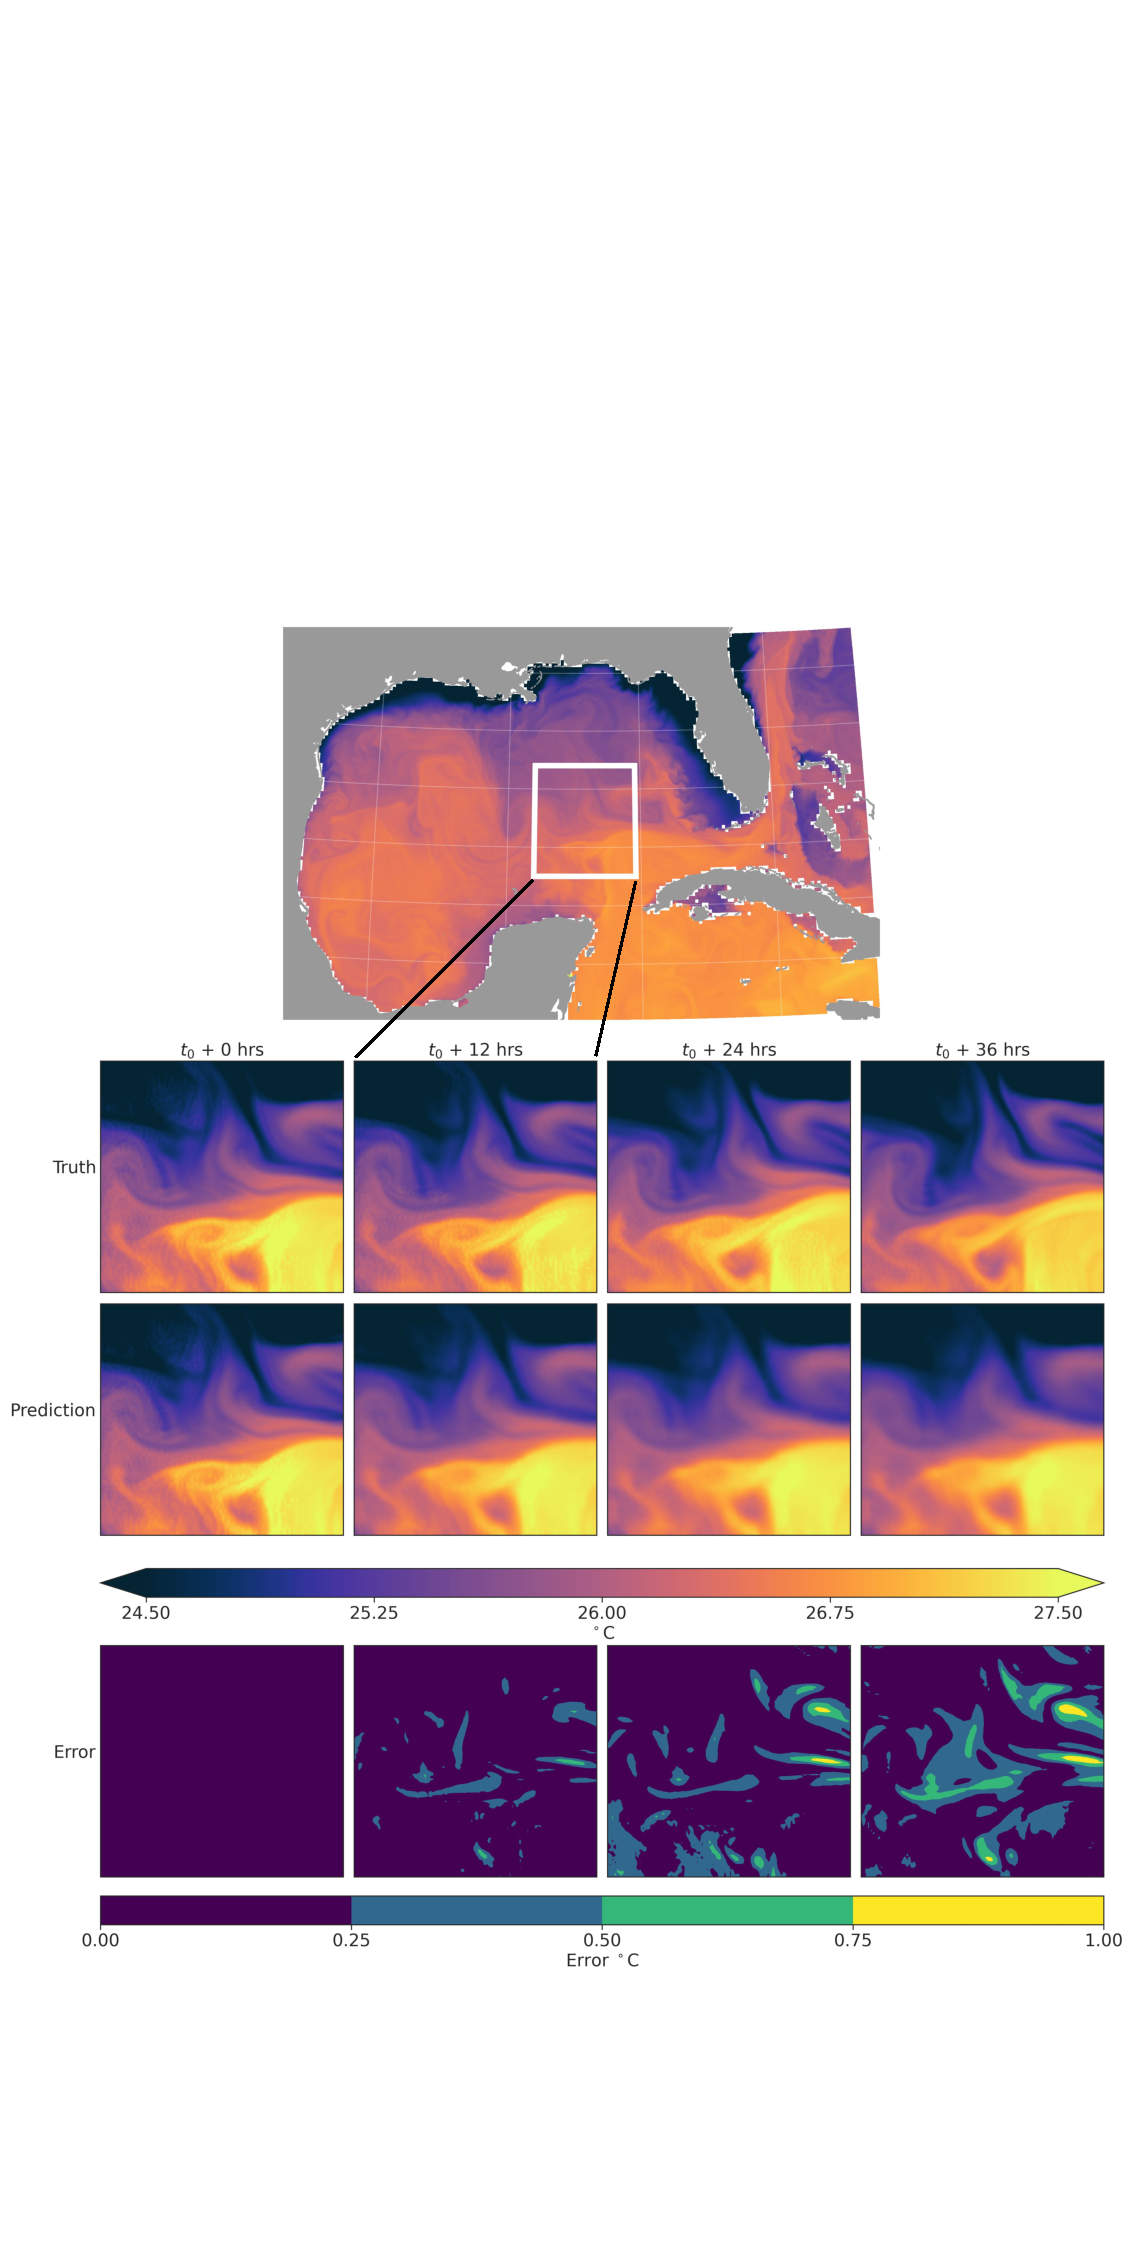
\includegraphics[width=.8\textwidth]{../figures/rc_gom_sst.pdf}
    \caption{A sample prediction of SSTs in the Gulf of Mexico at 1/25$^\circ$
        horizontal resolution.
        The upper row (Truth) shows the evolution of unseen test data from the
        Navy/HyCOM reanalysis product, and the middle row shows a prediction
        from the Reservoir Computing architecture described in \red{SECTION 2}.
        The bottom row (Error) shows the absolute value of the difference between the two.
        See \red{SECTION X} for a description of the training and testing data
        used.
    }
    \label{fig:gom_sst}
\end{figure}


